\documentclass[]{article}
\usepackage{lmodern}
\usepackage{amssymb,amsmath}
\usepackage{ifxetex,ifluatex}
\usepackage{fixltx2e} % provides \textsubscript
\ifnum 0\ifxetex 1\fi\ifluatex 1\fi=0 % if pdftex
  \usepackage[T1]{fontenc}
  \usepackage[utf8]{inputenc}
\else % if luatex or xelatex
  \ifxetex
    \usepackage{mathspec}
    \usepackage{xltxtra,xunicode}
  \else
    \usepackage{fontspec}
  \fi
  \defaultfontfeatures{Mapping=tex-text,Scale=MatchLowercase}
  \newcommand{\euro}{€}
\fi
% use upquote if available, for straight quotes in verbatim environments
\IfFileExists{upquote.sty}{\usepackage{upquote}}{}
% use microtype if available
\IfFileExists{microtype.sty}{%
\usepackage{microtype}
\UseMicrotypeSet[protrusion]{basicmath} % disable protrusion for tt fonts
}{}
\ifxetex
  \usepackage[setpagesize=false, % page size defined by xetex
              unicode=false, % unicode breaks when used with xetex
              xetex]{hyperref}
\else
  \usepackage[unicode=true]{hyperref}
\fi
\hypersetup{breaklinks=true,
            bookmarks=true,
            pdfauthor={},
            pdftitle={},
            colorlinks=true,
            citecolor=blue,
            urlcolor=blue,
            linkcolor=magenta,
            pdfborder={0 0 0}}
\urlstyle{same}  % don't use monospace font for urls
\usepackage{graphicx,grffile}
\makeatletter
\def\maxwidth{\ifdim\Gin@nat@width>\linewidth\linewidth\else\Gin@nat@width\fi}
\def\maxheight{\ifdim\Gin@nat@height>\textheight\textheight\else\Gin@nat@height\fi}
\makeatother
% Scale images if necessary, so that they will not overflow the page
% margins by default, and it is still possible to overwrite the defaults
% using explicit options in \includegraphics[width, height, ...]{}
\setkeys{Gin}{width=\maxwidth,height=\maxheight,keepaspectratio}
\setlength{\parindent}{0pt}
\setlength{\parskip}{6pt plus 2pt minus 1pt}
\setlength{\emergencystretch}{3em}  % prevent overfull lines
\providecommand{\tightlist}{%
  \setlength{\itemsep}{0pt}\setlength{\parskip}{0pt}}
\setcounter{secnumdepth}{0}

\date{}

% Redefines (sub)paragraphs to behave more like sections
\ifx\paragraph\undefined\else
\let\oldparagraph\paragraph
\renewcommand{\paragraph}[1]{\oldparagraph{#1}\mbox{}}
\fi
\ifx\subparagraph\undefined\else
\let\oldsubparagraph\subparagraph
\renewcommand{\subparagraph}[1]{\oldsubparagraph{#1}\mbox{}}
\fi
\title {Marker based localization \\ [10pt]
	Resizing  \\[25pt] Team members }
\author {Niharika Jayanthi \and Dheeraj Kamath}

\begin{document}
\maketitle
\begin{center}
	\begin{large}
		Under the guidance of\\
		\textbf{Sanam Shakya}\\
		\vspace{0.5in}
	\end{large}
\end{center}

\section{Goals}\label{goals}

\emph{\textbf{In this chapter we will learn :}}\\
* How to resize and image and apply basic filtering operations.\\
* We will see : \textbf{cv2.resize()}, \textbf{cv2.pyrDown()} ,
\textbf{cv2.pyrUp()}

\section{Theory}\label{theory}

\subsection{Resizing()}\label{resizing}

Scaling or resizing is basically changing the dimensions of the image
according to the specified scaling factor. Different interpolation
methods are used. Preferable interpolation methods are: *
\texttt{cv2.INTER\_AREA} for shrinking\\
 * \texttt{cv2.INTER\_CUBIC} (slow)\\
 * \texttt{cv2.INTER\_LINEAR} for zooming.

By default, interpolation method used is \texttt{cv2.INTER\_LINEAR} for
all resizing purposes.\\
As the size of an image is reduced or enlarged, the pixels that form the
image become increasingly visible, making the image appear ``soft'' if
pixels are averaged, or jagged if not.

\subsubsection{Function}\label{function}

The function is used in the following way:\\
\texttt{cv2.resize(src,\ dsize{[},\ dst{[},\ fx{[},\ fy{[},\ interpolation{]}{]}{]}{]})}

\subsubsection{Parameters:}\label{parameters}

\begin{itemize}
\tightlist
\item
  \textbf{src} -- input image.
\item
  \textbf{dst} -- output image; it has the size dsize (when it is
  non-zero) or the size computed from src.size(),fx, and fy; the type of
  dst is the same as of src.
\item
  \textbf{dsize} -- output image size; if it equals zero, it is computed
  as: \textbf{dsize = Size(round(fx\emph{source.cols), round =
  (fy}src.rows)} Either dsize or both fx and fy must be non-zero.
\item
  \textbf{fx} --scale factor along the horizontal axis; when it equals
  0, it is computed as\\
   \emph{\textbf{(double) dsize.width/src.cols}}
\item
  \textbf{fy} -- scale factor along the vertical axis; when it equals 0,
  it is computed as\\
  \emph{\textbf{(double) dsize.height/src.rows}}
\item
  \textbf{interpolation} --interpolation method:\\
   1. \texttt{INTER\_NEAREST} - a nearest-neighbor interpolation\\
   2. \texttt{INTER\_LINEAR} - a bilinear interpolation (used by
  default)\\
   3. \texttt{INTER\_AREA} - re-sampling using pixel area relation. It
  may be a preferred method for image decimation, as it gives
  moire'-free results. But when the image is zoomed, it is similar to
  the \texttt{INTER\_NEAREST} method.\\
   4. \texttt{INTER\_CUBIC} - a bicubic interpolation over 4x4 pixel
  neighborhood\\
   5. \texttt{INTER\_LANCZOS4} - a Lanczos interpolation over 8x8 pixel
  neighborhood
\end{itemize}

\subsection{Code}\label{code}

\begin{verbatim}
  #Import OpenCV, numpy and matplotlib
  import numpy
  import cv2
  import matplotlib.pyplot as plt

  #Read the image
  img = cv2.imread('lion.jpg')

  '''
  OpenCV represents RGB images as multi-dimensional NumPy arrays…but in reverse
  order!This means that images are actually represented in BGR order rather than
  RGB!
  '''
  img = cv2.cvtColor(img, cv2.COLOR_BGR2RGB)   #Convert to RGB

  #Resize()
  res = cv2.resize(img,None,fx=0.5, fy=0.5, interpolation = cv2.INTER_LINEAR)

  plt.figure(0)     #Create a new window
  plt.subplot(121),plt.imshow(img), plt.title('Original')
  plt.subplot(122), plt.imshow(res), plt.title('Resized')

  plt.show()        #Display the image
\end{verbatim}

Input image:\\
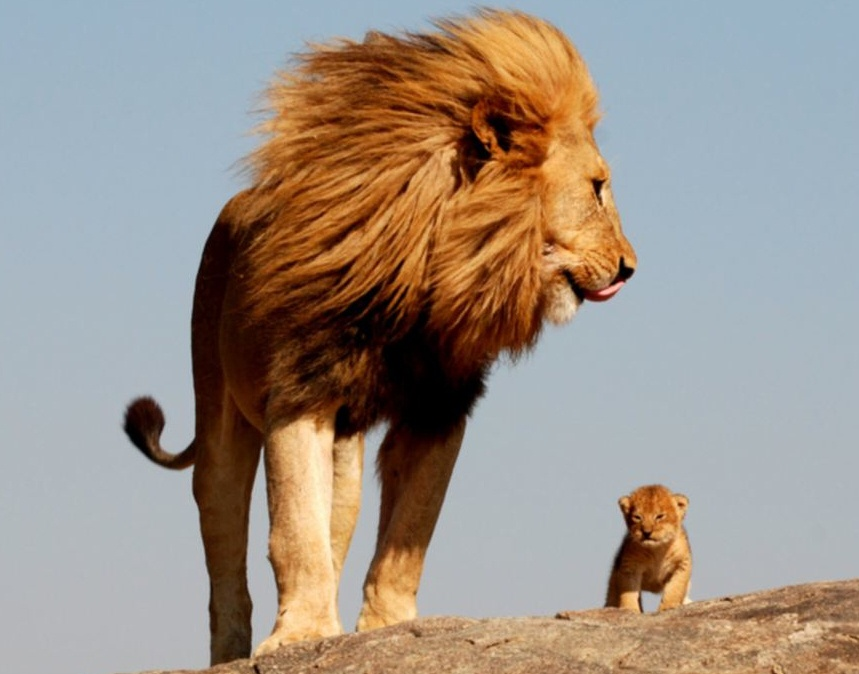
\includegraphics{original.jpg}

Output Image:\\
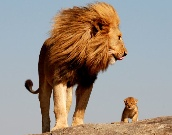
\includegraphics{res.jpg}

For better comparison, look at the table:
\begin{figure}
\centering
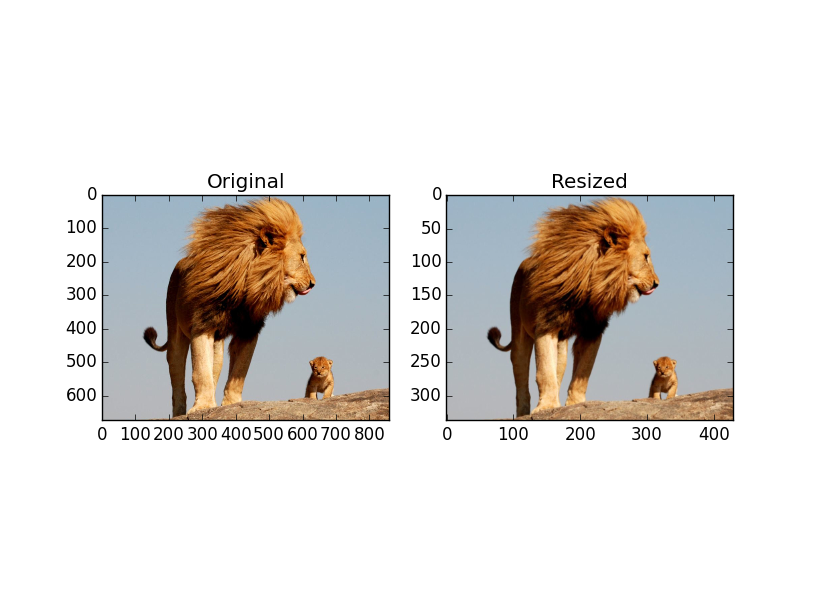
\includegraphics{resizecomp.png}
\end{figure}
\subsection{pyrUp() and pyrDown()}\label{pyrup-and-pyrdown}

OpenCV also offers inbuilt functions \texttt{pyrUp()} and
\texttt{pyrDown()}. Normally, we used to work with an image of constant size. But in some occasions, we need to work with images of different resolution of the same image. Set of images with different resolution are called Image Pyramids. There are two kinds of image pyramids
\begin{enumerate}
\item Gaussian pyramid
\item Laplacian pyramid
\end{enumerate}

Low resolution image is obtained by removing consecutive rows and
columns. Then each pixel in higher level is formed by the contribution
from 5 pixels in underlying level with Gaussian weights. By doing so, a
M x N image becomes M/2 x N/2 image.in this way area is reduced by 4
times. High resolution image is obtained by adding rows and columns
similarly. Area increases by four times. For downsizing the image we use
the function:

\texttt{cv2.pyrDown(src{[},\ dst{[},\ dstsize{[},\ borderType{]}{]}{]})}

For upsizing the image we use the function:

\texttt{cv2.pyrUp(src{[},\ dst{[},\ dstsize{[},\ borderType{]}{]}{]})}

\subsubsection{Parameters:}\label{parameters-1}

\begin{itemize}
\tightlist
\item
  \textbf{src} -- input image.
\item
  \textbf{dst} -- output image; it has the specified size and the same
  type as src.
\item
  \textbf{dstsize} -- size of the output image.
\item
  \textbf{borderType} -- Pixel extrapolation method (BORDER\_CONSTANT
  don't supported).
\end{itemize}

\section{Code}\label{code-1}

\begin{verbatim}
 #Import OpenCV, numpy and matplotlib
 import numpy
 import cv2
 import matplotlib.pyplot as plt


 #Read the image
 img = cv2.imread('lion.jpg')

 '''
 OpenCV represents RGB images as multi-dimensional NumPy arrays…but in reverse
 order!This means that images are actually represented in BGR order rather than
 RGB!
 '''
 img = cv2.cvtColor(img, cv2.COLOR_BGR2RGB)   #Convert to RGB

 #Resize()
 res1 = cv2.pyrUp(img,5)
 res2 = cv2.pyrDown(img,5)


 plt.figure(0)     #Create a new window
 plt.subplot(121),plt.imshow(img), plt.title('Original')
 plt.subplot(122), plt.imshow(res1), plt.title('pyrUp()')

 plt.figure(1)     #Create a new window
 plt.subplot(121),plt.imshow(img), plt.title('Original')
 plt.subplot(122), plt.imshow(res2), plt.title('pyrDown()')

 plt.show()        #Display the image
\end{verbatim}

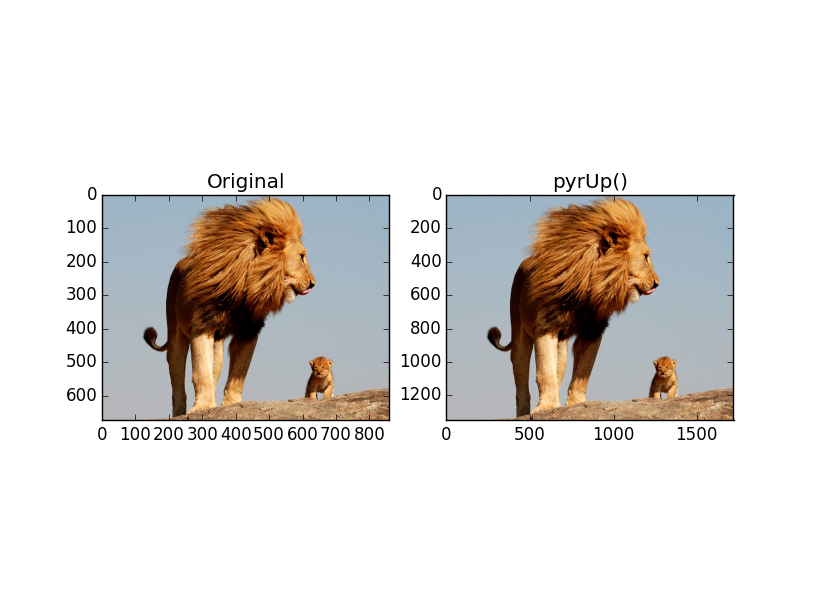
\includegraphics{pyrUp().png}
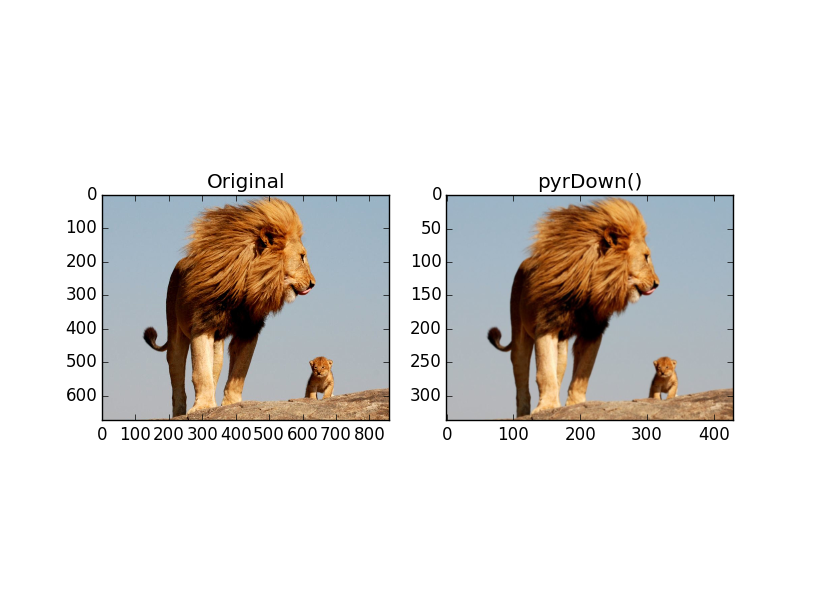
\includegraphics{pyrDown().png}

\section{Excercises}\label{excercises}

\begin{enumerate}
\def\labelenumi{\arabic{enumi}.}
\tightlist
\item
  Try to apply filtering operations on images before resizing and after
  resizing. Compare the results. You will find it fascinating.
\end{enumerate}

\subsection{Solution:}\label{solution}

\begin{verbatim}
 #Import OpenCV, numpy and matplotlib
 import numpy
 import cv2
 import matplotlib.pyplot as plt


 #Read the image
 img = cv2.imread('monalisa.jpg')

 '''
 OpenCV represents RGB images as multi-dimensional NumPy arrays…but in reverse
 order!This means that images are actually represented in BGR order rather than
 RGB!
 '''
 img = cv2.cvtColor(img, cv2.COLOR_BGR2RGB)   #Convert to RGB

 #Resize()
 res = cv2.resize(img,None,fx=0.2, fy=0.2, interpolation = cv2.INTER_LINEAR)
 
 #Applying filters on image resized using resize()
 r1_blur = cv2.medianBlur(res,5)

 #Applying filters on original image
 nr_blur = cv2.medianBlur(img,5)

 #Downsizing the image
 ds = cv2.pyrDown(img, 5)

 #Applying filters on downsized image using pyrDown()
 r2_blur = cv2.medianBlur(ds,5)


 plt.figure("Compare")         #Create a new window
 plt.subplot(221),plt.imshow(img), plt.title('Original image')
 plt.xticks([]), plt.yticks([])
 plt.subplot(222),plt.imshow(nr_blur),plt.title('Median Blur without resize')
 plt.xticks([]), plt.yticks([])
 plt.subplot(223),plt.imshow(r1_blur),plt.title('Median Blur after resize()')
 plt.xticks([]), plt.yticks([])
 plt.subplot(224),plt.imshow(r2_blur),plt.title('Median Blur after pyrDown()')
 plt.xticks([]), plt.yticks([])
 plt.show()
\end{verbatim}

\begin{figure}[htbp]
\centering
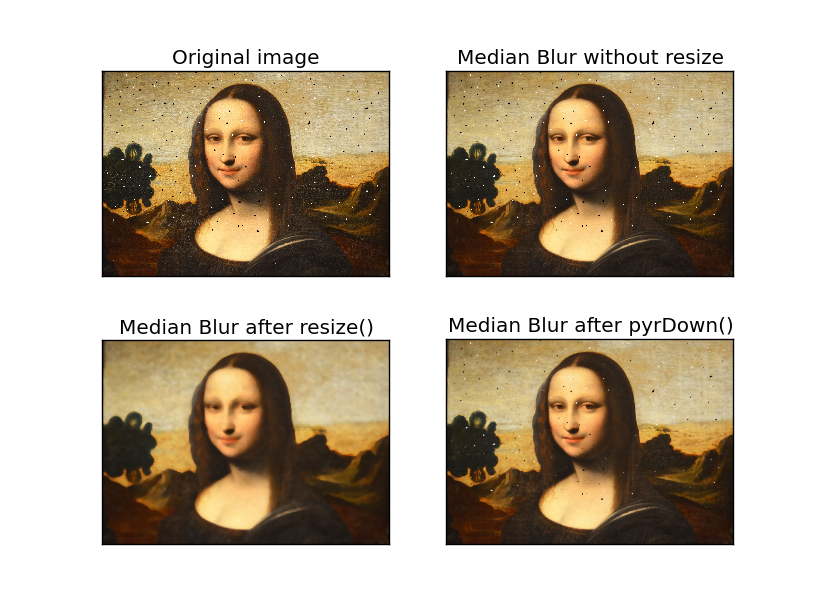
\includegraphics{compare.png}
\caption{Output Image}
\end{figure}

\section{References}\label{references}

\begin{enumerate}
\def\labelenumi{\arabic{enumi}.}
\tightlist
\item
  \href{http://opencv-python-tutroals.readthedocs.org/en/latest/py\_tutorials/
  py\_imgproc/py\_pyramids/py\_pyramids.html\#pyramids}{Resizing - opencv-python tutorials}
\item
  \href{http://docs.opencv.org/modules/imgproc/doc/filtering.html\#pyrdown}{pyrDown - opencv docs}
\end{enumerate}

\end{document}
